\section{Общее задание}

\subsection{Компьютер 1}
\begin{itemize}
    \item Сеть 1--2

    \begin{tabular}{ll}
        IPv4 & \texttt{5.6.12.1/24}         \\
        IPv6 & \texttt{::ffff:5.6.12.1/120} \\
    \end{tabular}

    \item Сеть 1--3

    \begin{tabular}{ll}
        IPv4 & \texttt{5.6.13.1/24}         \\
        IPv6 & \texttt{::ffff:5.6.13.1/120} \\
    \end{tabular}
\end{itemize}

Конфигурация:
\begin{verbatim}
ip link set enp0s8 down
ip link set enp0s9 down

sysctl -w net.ipv4.ip_forward=1
sysctl -w net.ipv4.conf.enp0s8.rp_filter=0
sysctl -w net.ipv4.conf.enp0s9.rp_filter=0

ip    a flush enp0s8
ip -6 a flush enp0s8
ip    a flush enp0s9
ip -6 a flush enp0s9
ip    r flush default
ip -6 r flush default

ip link set enp0s8 up
ip    a a        5.6.12.1/24  dev enp0s8
ip -6 a a ::ffff:5.6.12.1/120 dev enp0s8

ip link set enp0s9 up
ip    a a        5.6.13.1/24  dev enp0s9
ip -6 a a ::ffff:5.6.13.1/120 dev enp0s9

ip    r a default via        5.6.12.2
ip -6 r a default via ::ffff:5.6.12.2
\end{verbatim}

Настройки \texttt{iptables}:
\begin{verbatim}
iptables  -F
ip6tables -F

iptables -A OUTPUT -s 5.6.12.1 -j REJECT
iptables -A INPUT  -p icmp -m length --length 1001: -m ttl --ttl-lt 10 -j REJECT
iptables -A OUTPUT -p icmp -m length --length 1001: -m ttl --ttl-lt 10 -j REJECT

ip6tables -A OUTPUT -s ::ffff:5.6.12.1 -j REJECT
ip6tables -A INPUT  -p icmpv6 -m length --length 1001: -j REJECT
ip6tables -A OUTPUT -p icmpv6 -m length --length 1001: -j REJECT
\end{verbatim}

\subsection{Компьютер 2}
\begin{itemize}
    \item Сеть 1-2

    \begin{tabular}{ll}
        IPv4 & \texttt{5.6.12.2/24}     \\
        IPv6 & \texttt{::ffff:5.6.12.2} \\
    \end{tabular}

    \item Сеть 2-3

    \begin{tabular}{ll}
        IPv4 & \texttt{5.6.23.2/24}     \\
        IPv6 & \texttt{::ffff:5.6.23.2} \\
    \end{tabular}
\end{itemize}

Конфигурация:
\begin{verbatim}
ip link set enp0s8 down
ip link set enp0s9 down

sysctl -w net.ipv4.ip_forward=1
sysctl -w net.ipv4.conf.enp0s8.rp_filter=0
sysctl -w net.ipv4.conf.enp0s9.rp_filter=0

ip    a flush enp0s8
ip -6 a flush enp0s8
ip    a flush enp0s9
ip -6 a flush enp0s9
ip    r flush default
ip -6 r flush default

ip link set enp0s8 up
ip    a a        5.6.12.2/24  dev enp0s8
ip -6 a a ::ffff:5.6.12.2/120 dev enp0s8

ip link set enp0s9 up
ip    a a        5.6.23.2/24  dev enp0s9
ip -6 a a ::ffff:5.6.23.2/120 dev enp0s9

ip    r a default via        5.6.23.3
ip -6 r a default via ::ffff:5.6.23.3
\end{verbatim}

Настройки \texttt{iptables} --- пустые.

\subsection{Компьютер 3}
\begin{itemize}
    \item Сеть 1-3

    \begin{tabular}{ll}
        IPv4 & \texttt{5.6.13.3/24}     \\
        IPv6 & \texttt{::ffff:5.6.13.3} \\
    \end{tabular}

    \item Сеть 2-3

    \begin{tabular}{ll}
        IPv4 & \texttt{5.6.23.3/24}     \\
        IPv6 & \texttt{::ffff:5.6.23.3} \\
    \end{tabular}

    \item Сеть 3-4

    \begin{tabular}{ll}
        IPv4 & \texttt{5.6.34.3/24}     \\
        IPv6 & \texttt{::ffff:5.6.34.3} \\
    \end{tabular}
\end{itemize}

Конфигурация:
\begin{verbatim}
ip link set enp0s8  down
ip link set enp0s9  down
ip link set enp0s10 down

sysctl -w net.ipv4.ip_forward=1
sysctl -w net.ipv4.conf.enp0s8.rp_filter=0
sysctl -w net.ipv4.conf.enp0s9.rp_filter=0
sysctl -w net.ipv4.conf.enp0s10.rp_filter=0

ip    a flush enp0s8
ip -6 a flush enp0s8
ip    a flush enp0s9
ip -6 a flush enp0s9
ip    a flush enp0s10
ip -6 a flush enp0s10
ip    r flush default
ip -6 r flush default

ip link set enp0s8 up
ip    a a        5.6.13.3/24  dev enp0s8
ip -6 a a ::ffff:5.6.13.3/120 dev enp0s8

ip link set enp0s9 up
ip    a a        5.6.23.3/24  dev enp0s9
ip -6 a a ::ffff:5.6.23.3/120 dev enp0s9

ip link set enp0s9 up
ip    a a        5.6.34.3/24  dev enp0s10
ip -6 a a ::ffff:5.6.34.3/120 dev enp0s10

ip    r a default via        5.6.23.2
ip -6 r a default via ::ffff:5.6.23.2
\end{verbatim}

Настройки \texttt{iptables} --- пустые.

\subsection{Компьютер 4}
\begin{itemize}
    \item Сеть 3-4

    \begin{tabular}{ll}
        IPv4 & \texttt{5.6.34.4/24}     \\
        IPv6 & \texttt{::ffff:5.6.34.4} \\
    \end{tabular}
\end{itemize}

Конфигурация:
\begin{verbatim}
ip link set enp0s8 down

sysctl -w net.ipv4.ip_forward=1
sysctl -w net.ipv4.conf.enp0s8.rp_filter=0

ip    a flush enp0s8
ip -6 a flush enp0s8
ip    r flush default
ip -6 r flush default

ip link set enp0s8 up
ip    a a        5.6.34.4/24  dev enp0s8
ip -6 a a ::ffff:5.6.34.4/120 dev enp0s8

ip    r a default via        5.6.34.3
ip -6 r a default via ::ffff:5.6.34.3
\end{verbatim}

Настройки \texttt{iptables}:
\begin{verbatim}
iptables  -F
ip6tables -F

iptables -A OUTPUT -p tcp --dport 4001 -j REJECT
iptables -A INPUT  -p udp --dport 4001 -j REJECT
iptables -A INPUT  -d 5.6.34.4 -j REJECT
iptables -A INPUT  -p icmp -m length --length 1001: -m ttl --ttl-lt 10 -j REJECT
iptables -A OUTPUT -p icmp -m length --length 1001: -m ttl --ttl-lt 10 -j REJECT

ip6tables -A OUTPUT -p tcp --dport 4001 -j REJECT
ip6tables -A INPUT  -p udp --dport 4001 -j REJECT
ip6tables -A INPUT  -d ::ffff:5.6.34.4 -j REJECT
ip6tables -A INPUT  -p icmpv6 -m length --length 1001: -j REJECT
ip6tables -A OUTPUT -p icmpv6 -m length --length 1001: -j REJECT
\end{verbatim}

\subsection{Скриншоты выполнения}
\texttt{ncat} без \texttt{iptables}

\begin{center}
    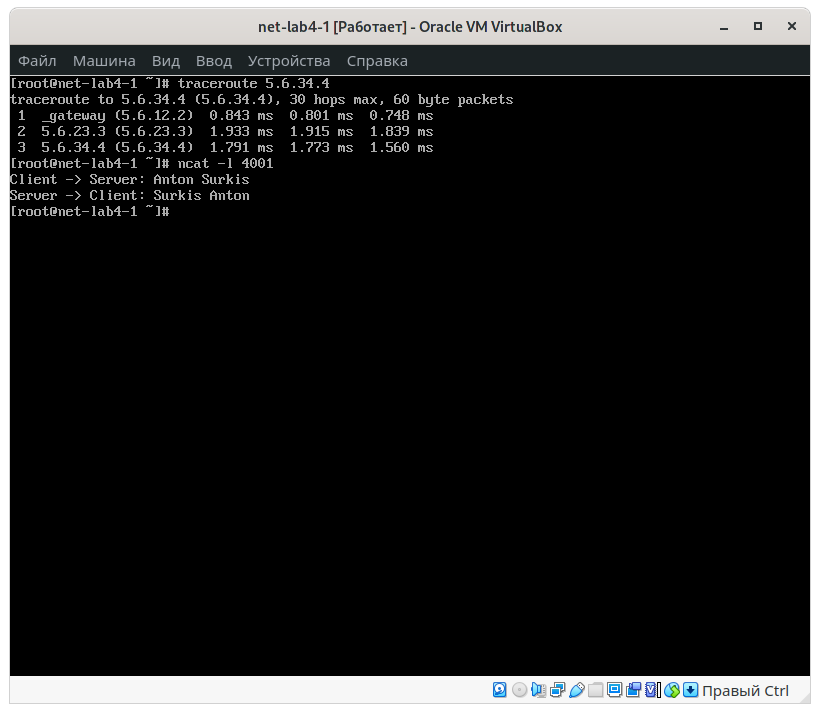
\includegraphics[width=.49\textwidth]{screenshots/base-ncat-A}
    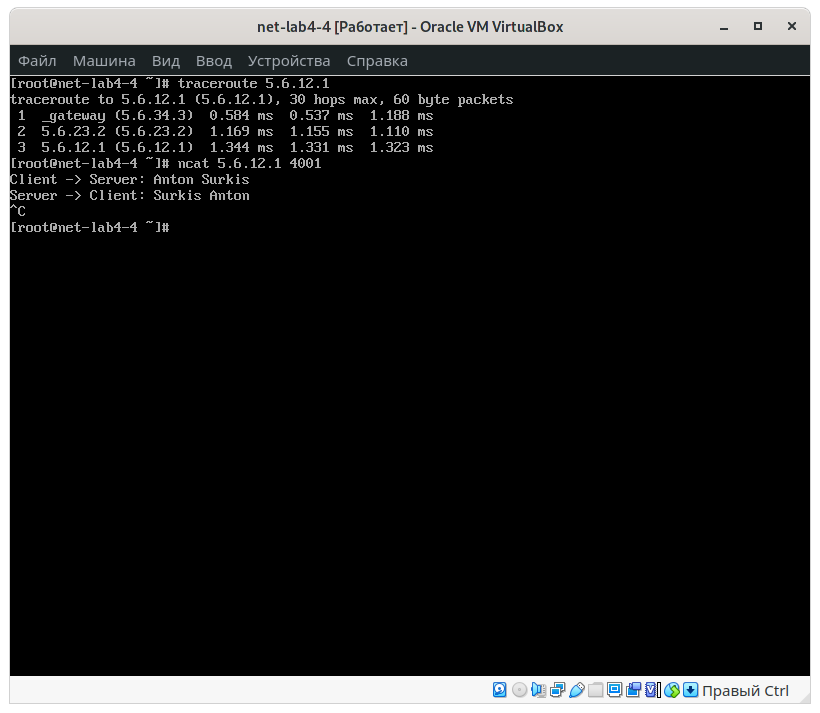
\includegraphics[width=.49\textwidth]{screenshots/base-ncat-B}
\end{center}

\texttt{ping} с полным \texttt{iptables}

\begin{center}
    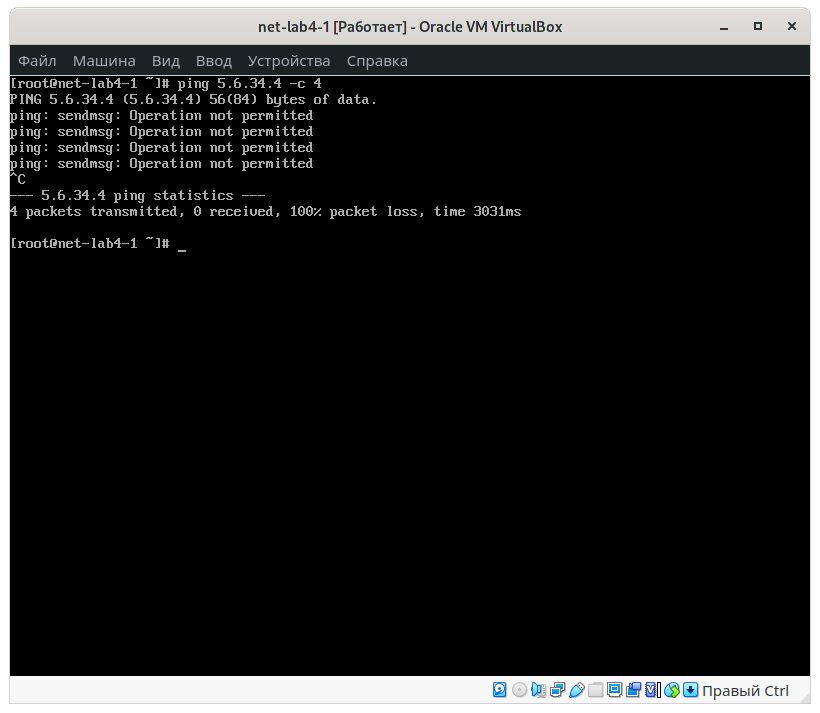
\includegraphics[width=.49\textwidth]{screenshots/base-ping-blocked-A}
    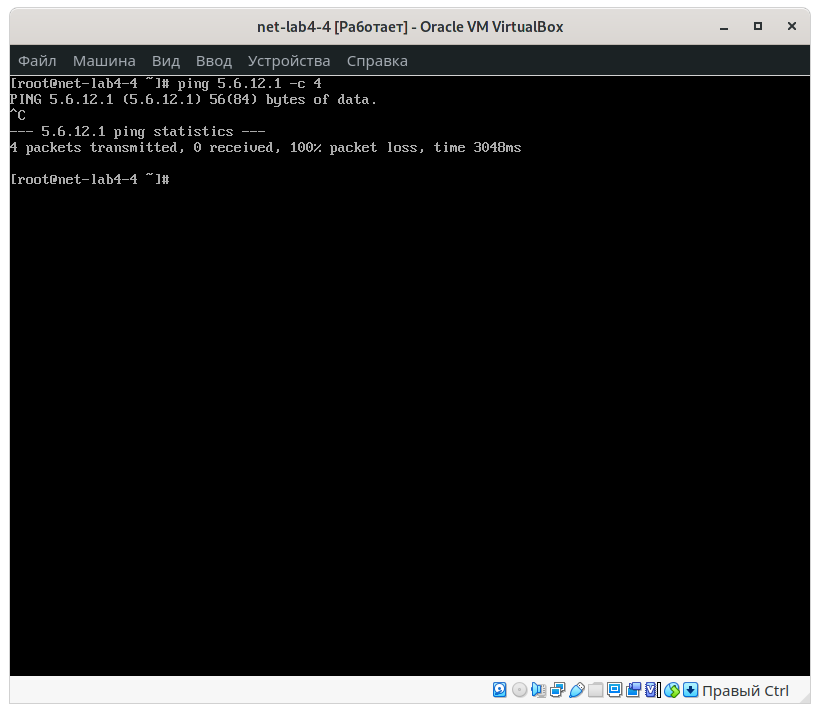
\includegraphics[width=.49\textwidth]{screenshots/base-ping-blocked-B}
\end{center}

Как можно заметить, отправка и прием пакетов невозможны,
т.к. эффективно запрещена любая передача пакетов.
Уберем эти 2 правила:

\begin{center}
    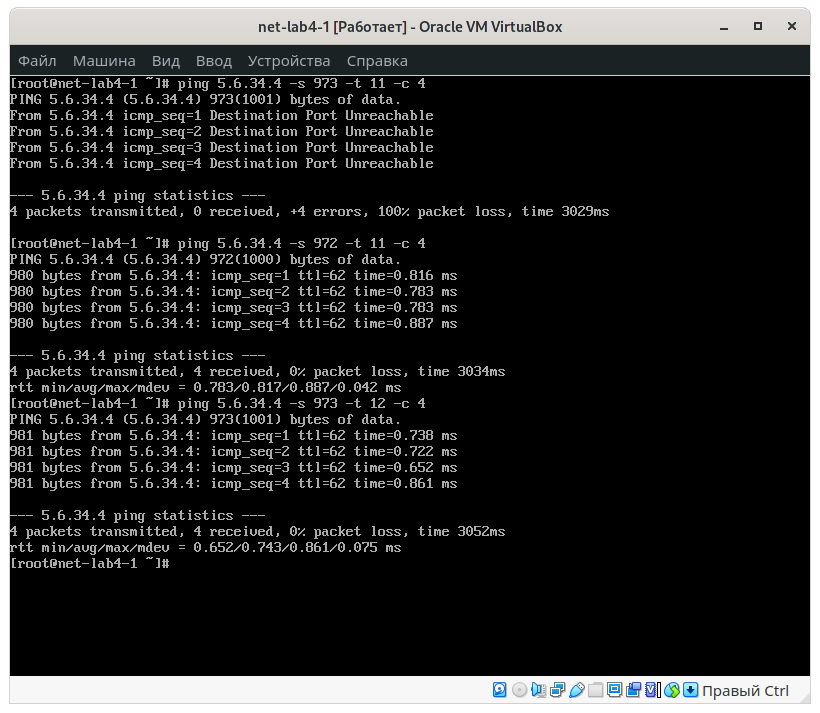
\includegraphics[width=.49\textwidth]{screenshots/base-ping-iptables-A}
    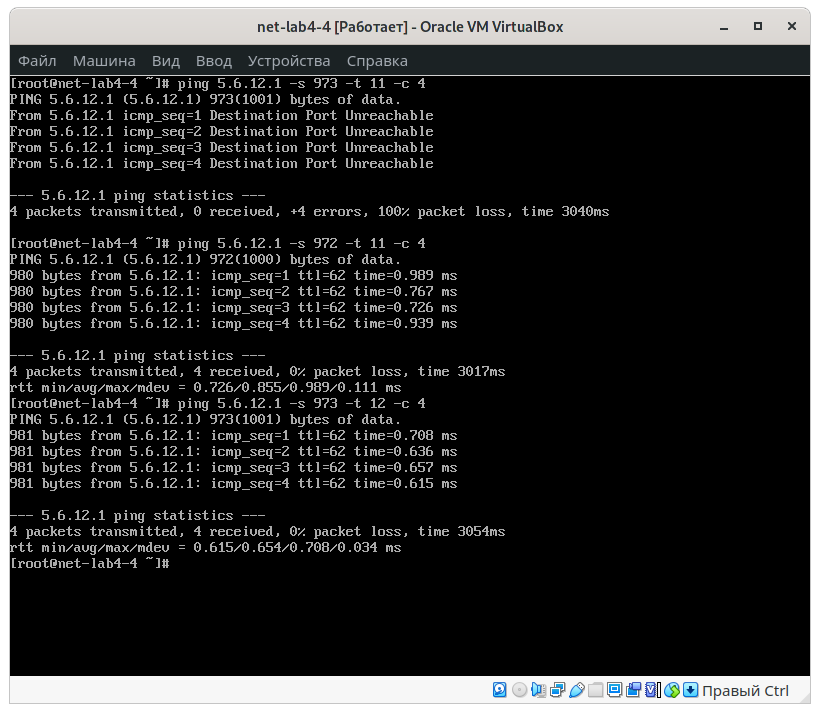
\includegraphics[width=.49\textwidth]{screenshots/base-ping-iptables-B}
\end{center}

\texttt{ncat} по разным протоколам:

\begin{center}
    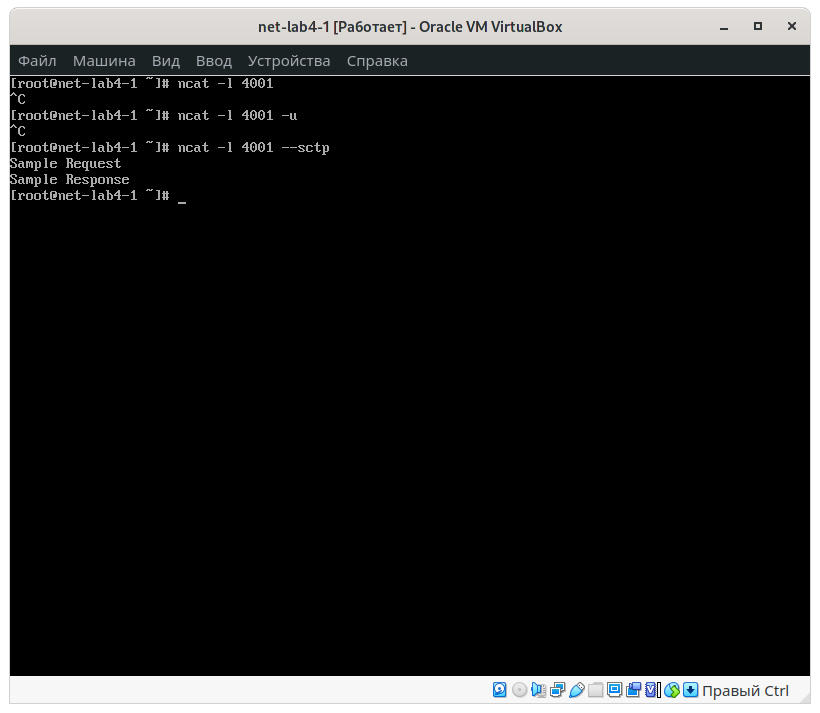
\includegraphics[width=.49\textwidth]{screenshots/base-ncat-iptables-A}
    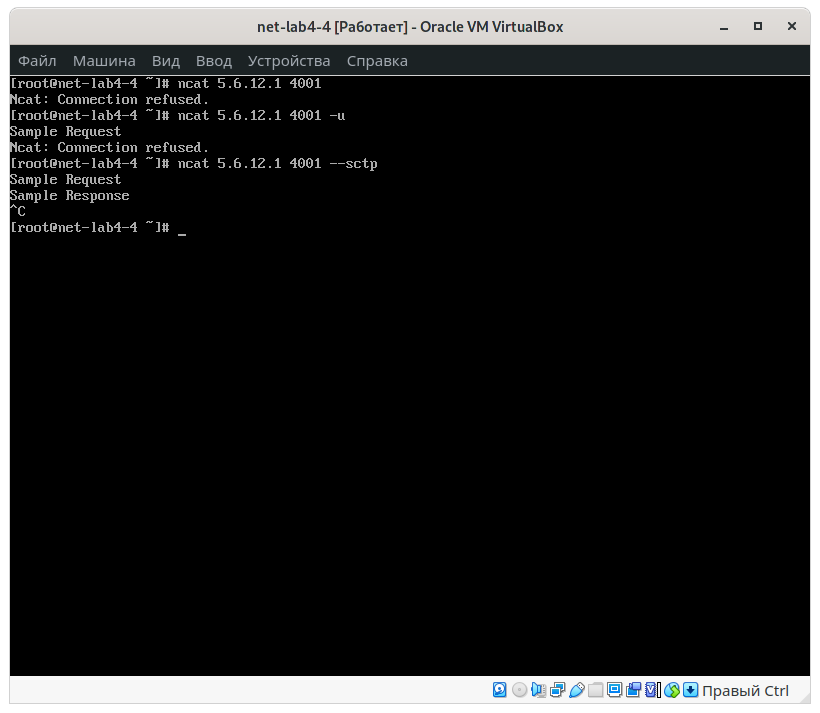
\includegraphics[width=.49\textwidth]{screenshots/base-ncat-iptables-B}
\end{center}
